\documentclass[conference,a4paper]{IEEEtran}
\usepackage{graphicx,booktabs,amsmath,multirow,url,xcolor}
\usepackage{newtxtext,newtxmath}
\usepackage[hidelinks]{hyperref}
\usepackage{tikz}
\usetikzlibrary{positioning,arrows.meta,fit}
% Shared metadata for the proposal and the report. Fill these in, then rebuild both PDFs.
\newcommand{\institute}{[Institute name]}
\newcommand{\course}{[Course code]: Deep Learning}
\newcommand{\repourl}{\url{https://github.com/[team]/diabetic-retinopathy-grading}}

\graphicspath{{figures/}}
\newcommand{\pmci}[2]{{\scriptsize[#1, #2]}}

\begin{document}
\title{Ordinal Diabetic Retinopathy Grading with Vision Transformers and CNNs on Free-Tier GPUs: Internal and External Validation for Mass Screening}

\author{\IEEEauthorblockN{Abhinav Shukla (230101002), Amit Kumar (230101021), Shaurya Shakya (230101119),\\
Nitin Gupta (230101083), Utkarsh Kumar (230101147), Amit Usara (230101023), Somil Gupta (230101135),\\
Krishna Kumar Gupta (230101068), Saurabh Mishra (230101116), Shreyansh Anand (230101128)}
\IEEEauthorblockA{Department of Computer Science and Engineering, \institute\\ \course\quad Code: \repourl}}

\maketitle

\begin{abstract}
We grade retinal fundus photographs into the five ICDR severity levels of diabetic retinopathy (DR) to support mass screening camps.
The whole pipeline runs within the Kaggle free tier: two T4 GPUs, 12-hour sessions and a 20\,GB output limit.
It preprocesses the original 82\,GB EyePACS archive in place, without extracting it, and stores 768\,px fundus crops.
It removes conflicting near-duplicates from APTOS-2019 and splits the data by patient.
We fine-tune a ViT-B/16 and a ResNet-50 at 512\,px with a cumulative ordinal head, square-root class-rebalanced sampling and ordinal label smoothing.
At inference we use four-view test-time augmentation (TTA), whose spread doubles as an uncertainty flag.
Grade cut-offs are tuned for quadratic weighted kappa (QWK); a separate screening cut-off is fixed at 90\% referable-DR sensitivity on validation data.
Fusing the two models and the patient's two eyes gives QWK 0.838 on the 42,666-image EyePACS Private test set, with referable-DR AUC 0.955.
On the external Messidor-2 set (adjudicated grades, never used for training or tuning) it gives QWK 0.843 and AUC 0.969.
The ViT and the CNN are tied on EyePACS (0.808 vs.\ 0.803), but the ViT transfers better to Messidor-2 (0.840 vs.\ 0.819).
The CNN's screening cut-off also loses specificity on the new site (0.61 vs.\ 0.78), a concrete instance of the domain-shift risk we discuss with the other clinical limitations.
We also report and fix an engineering pitfall: \texttt{nn.DataParallel} defeats cuDNN's thread-local plan cache, which made CNN training several times slower and leaked host memory.
\end{abstract}

\begin{IEEEkeywords}
diabetic retinopathy, ordinal classification, vision transformer, external validation, class imbalance, label noise, test-time augmentation
\end{IEEEkeywords}

\section{Introduction}
Diabetic retinopathy affects an estimated 22.3\% of people with diabetes, and the number of adults with DR is projected to reach 160.5 million by 2045~\cite{teo}.
Vision loss is largely preventable if referable disease is caught early.
Early DR, however, is asymptomatic, so systematic fundus photography is needed, and screening camps in low-resource settings produce far more images than retina specialists can grade.
Automated grading with deep networks reached specialist-level accuracy in retrospective studies~\cite{gulshan,krause}, and autonomous systems have been cleared after prospective trials~\cite{abramoff}.
Field deployments still show how fragile the image-to-decision chain is under real conditions~\cite{beede}.

We build a screening tool that maps a fundus photograph to the five-level International Clinical DR (ICDR) scale~\cite{icdr}: 0 none, 1 mild, 2 moderate, 3 severe non-proliferative DR, 4 proliferative DR (PDR).
Because the grades are ordered and mistakes between distant grades are worse, we treat the task as ordinal classification and report the quadratic weighted kappa (QWK)~\cite{cohen}.
For referral we also report sensitivity and specificity for \emph{referable} DR (rDR, grade $\ge$2) and \emph{vision-threatening} DR (VTDR, grade $\ge$3).

Three practical difficulties shape the design.
\begin{enumerate}
\item \textbf{Small lesions vs.\ resolution.} Microaneurysms span only a few pixels even in the original 3--5\,MP images. CNNs can be run at high resolution cheaply, but ViT cost grows quadratically in the number of tokens.
\item \textbf{Imbalance and label noise.} About 73\% of EyePACS images are grade 0. Its labels come from single graders, whose agreement is only moderate~\cite{krause}.
\item \textbf{Compute.} Everything must run on the Kaggle free tier: about 30 GPU-hours per week on 2$\times$T4, 12\,h sessions, 20\,GB of output and a $\sim$500-file output limit. That is less than the 82\,GB original archive.
\end{enumerate}

\textbf{Contributions.}
\begin{enumerate}
\item A reproducible three-notebook pipeline that fits the free tier. It streams EyePACS directly out of its split zip parts, removes duplicate and conflicting APTOS labels, and makes patient-grouped splits.
\item A controlled CNN vs.\ ViT comparison at 512\,px, using the same ordinal formulation, imbalance handling, TTA and operating-point selection for both.
\item Internal evaluation on 53,571 EyePACS test images (including the 42,666-image Private split, for comparison with the literature) and \emph{external} validation on Messidor-2 with adjudicated grades. We report per-grade confusion matrices, bootstrap CIs and a screening operating point.
\item Ensembling and paired-eye fusion, both fitted on validation data only. Together they lift Private-test QWK from 0.808 to 0.838.
\item A clinical-limitations analysis, and an engineering note on multi-GPU training that explains a several-fold CNN slowdown on current PyTorch.
\end{enumerate}

\section{Related Work}
\textbf{Deep learning for DR screening.}
Gulshan \emph{et al.}~\cite{gulshan} trained Inception-v3 on 128k images, each graded 3--7 times. They reported rDR AUC 0.991 on EyePACS-1 and 0.990 on Messidor-2.
Reproducing this with public data only, Voets \emph{et al.}~\cite{voets} obtained AUC 0.951 on the Kaggle EyePACS test and 0.853 on Messidor-2. That gap is the cost of noisy labels and of an external domain.
Krause \emph{et al.}~\cite{krause} showed that individual specialists' kappa against an adjudicated reference ranges from 0.82 to 0.91. They also found that tuning on adjudicated grades and using higher-resolution inputs raised AUC from 0.934 to 0.986. Their adjudicated Messidor-2 grades are our external reference.
IDx-DR, the first FDA-authorised autonomous DR system, reported 87.2\% sensitivity and 90.7\% specificity in a prospective primary-care trial~\cite{abramoff}.
Beede \emph{et al.}~\cite{beede} documented how image quality, lighting and workflow degrade a deployed system in Thai clinics.

\textbf{Kaggle-era methods.}
The 2015 Kaggle winner, Graham~\cite{graham}, reached QWK 0.849 on the Private test. He subtracted a Gaussian-blurred local average colour to normalise illumination, trained at high resolution and blended features from both eyes.
Later work added lesion-aware attention (Zoom-in-Net~\cite{zoomin}, 0.854; AFN~\cite{afn}, 0.859) and category attention for imbalance (CABNet~\cite{cabnet}).
Huang \emph{et al.}~\cite{huang} ran a controlled ablation of ResNet-50 on the same EyePACS split. They found that 512$\rightarrow$768\,px adds $\sim$0.01 QWK, an MSE (regression) objective beats cross-entropy by $\sim$0.02, and Graham or CLAHE preprocessing slightly \emph{hurts} a pretrained CNN.
In their study, instance-balanced sampling beat class-balanced sampling, and paired-eye feature fusion was the largest late gain (+0.027). They reached 0.858 for a single model and 0.863 for an ensemble.

\textbf{Ordinal regression and imbalance.}
Frank and Hall~\cite{frankhall} decompose a $K$-class ordinal problem into $K-1$ binary ``$y>k$'' problems. CORAL~\cite{coral} shares weights across these to make the predictions rank-consistent.
Kang \emph{et al.}~\cite{kang} analyse instance-, class- and square-root-balanced sampling for long-tailed recognition. Label smoothing~\cite{smoothing} is a cheap regulariser against noisy targets.

\textbf{Transformers for retinal images.}
ViT~\cite{vit} tokenises 16$\times$16 patches and needs large-scale pretraining; we use AugReg weights~\cite{augreg}.
Lesion-Aware Transformers~\cite{lat} use lesion queries for DR grading. RETFound~\cite{retfound} is a ViT-L foundation model pretrained with MAE on 1.6M retinal images.
Its 224\,px input and gated weights make it a poor fit for our resolution and compute constraints, so we fine-tune a ViT-B/16 at 512\,px instead (1024 tokens).

\section{Data}
\subsection{Sources}
Table~\ref{tab:data} lists the datasets.
\begin{itemize}
\item \textbf{EyePACS}~\cite{eyepacs} (Kaggle 2015) contributes 35,126 labelled training images and 53,576 test images from US primary-care screening, taken with many different cameras. The test labels were released after the competition, together with the Public/Private split used by the leaderboard and by later papers.
\item \textbf{APTOS-2019} adds 3,662 labelled images from Aravind Eye Hospital (India).
\item \textbf{Messidor-2}~\cite{messidor} (France, Topcon TRC NW6, 1,748 images) serves as the external test set. We use the adjudicated grades of Krause \emph{et al.}~\cite{krause} and exclude the 4 ungradable images.
\end{itemize}
All sources are public on Kaggle. The two competitions require accepting their rules.

\begin{table}[t]
\centering\caption{Datasets and their role.}\label{tab:data}
\footnotesize
\begin{tabular}{@{}llrl@{}}
\toprule
Dataset & Origin & Images & Role\\
\midrule
EyePACS train & USA, many cameras & 35,121 & train / val\\
APTOS-2019 & India & 3,487 & train / val\\
EyePACS test & USA, many cameras & 53,571 & internal test\\
\quad Private split & & 42,666 & vs.\ literature\\
Messidor-2 & France, Topcon & 1,744 & \textbf{external}\\
\bottomrule
\end{tabular}
\end{table}

\subsection{Preprocessing within free-tier limits}
The original EyePACS archive ($\sim$82\,GB) is stored as byte-split zip parts (\texttt{train.zip.001}--\texttt{.005}, \texttt{test.zip.001}--\texttt{.007}). That exceeds Kaggle's working disk.
We wrap the parts in a seekable virtual file so that Python's \texttt{zipfile} can read members in place, and process them with one worker per CPU (Fig.~\ref{fig:pipeline}).
JPEGs are decoded at reduced scale through libjpeg's DCT scaling (PIL \texttt{draft}), about 4$\times$ faster than a full decode.
Each image is tight-cropped to the fundus disc by thresholding the maximum channel (15/255), padded to a centred square, and resized to \textbf{768\,px}.
Ten images without a detectable fundus (5 train, 5 test) were skipped.
Images are written uncompressed into one zip shard per source, because Kaggle limits notebook output to about 500 files. The shards total about 10\,GB.
Storing 768\,px leaves headroom: at the 512\,px training size, microaneurysms are still about 2--4\,px.
Enhancement is applied at load time, so it can be ablated.
Ben Graham enhancement~\cite{graham} computes $I' = 4I - 4\,G_{\sigma}*I + 128$ with $\sigma = s/30$ for image size $s$. It then clips to a disc of radius $0.45s$ to remove the bright rim artefact (Fig.~\ref{fig:samples}).

\begin{figure*}[t]
\centering
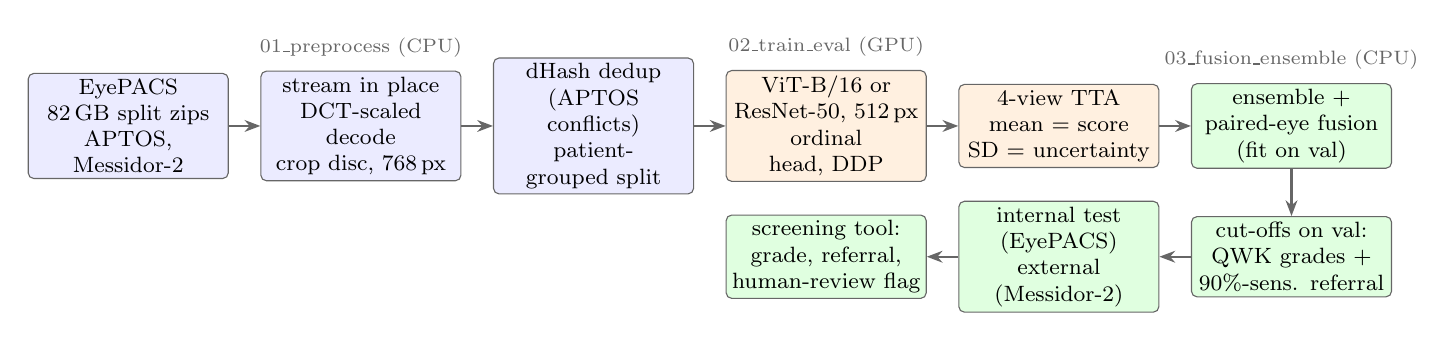
\begin{tikzpicture}[node distance=3mm and 4mm, every node/.style={font=\footnotesize, align=center},
  box/.style={draw=black!60, rounded corners=2pt, fill=#1, minimum height=9mm, inner sep=2pt, text width=24mm},
  arr/.style={-{Stealth[length=2mm]}, thick, draw=black!60}]
\node[box=blue!8] (raw) {EyePACS 82\,GB split zips\\APTOS, Messidor-2};
\node[box=blue!8, right=of raw] (crop) {stream in place\\DCT-scaled decode\\crop disc, 768\,px};
\node[box=blue!8, right=of crop] (clean) {dHash dedup\\(APTOS conflicts)\\patient-grouped split};
\node[box=orange!12, right=of clean] (train) {ViT-B/16 or\\ResNet-50, 512\,px\\ordinal head, DDP};
\node[box=orange!12, right=of train] (tta) {4-view TTA\\mean = score\\SD = uncertainty};
\node[box=green!12, right=of tta] (fuse) {ensemble +\\paired-eye fusion\\(fit on val)};
\node[box=green!12, below=6mm of fuse] (op) {cut-offs on val:\\QWK grades +\\90\%-sens. referral};
\node[box=green!12, left=of op] (eval) {internal test\\(EyePACS)\\external (Messidor-2)};
\node[box=green!12, left=of eval] (screen) {screening tool:\\grade, referral,\\human-review flag};
\foreach \a/\b in {raw/crop, crop/clean, clean/train, train/tta, tta/fuse, fuse/op, op/eval, eval/screen} \draw[arr] (\a) -- (\b);
\node[font=\scriptsize, text=black!60, above=0.5mm of crop] {01\_preprocess (CPU)};
\node[font=\scriptsize, text=black!60, above=0.5mm of train] {02\_train\_eval (GPU)};
\node[font=\scriptsize, text=black!60, above=0.5mm of fuse] {03\_fusion\_ensemble (CPU)};
\end{tikzpicture}
\caption{End-to-end pipeline. Three Kaggle notebooks; only the second uses GPU quota.}
\label{fig:pipeline}
\end{figure*}

\begin{figure*}[t]
\centering
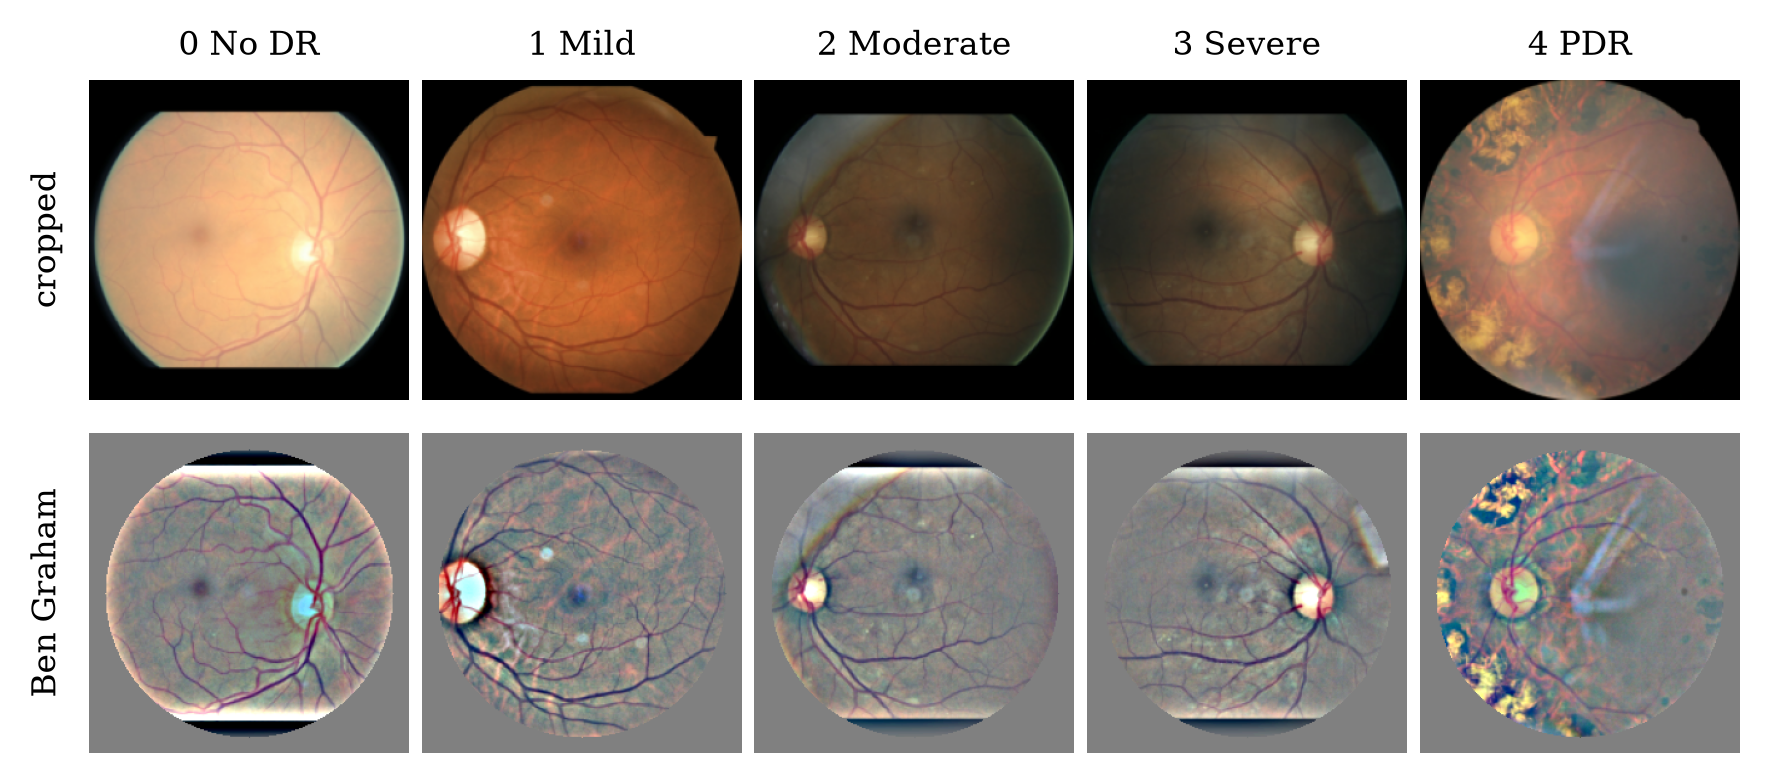
\includegraphics[width=0.86\linewidth]{fig_samples.png}
\caption{One stored 768\,px crop per grade (top) and the same image after Ben Graham enhancement (bottom). The enhancement removes illumination and colour differences between cameras and makes exudates, haemorrhages and new vessels stand out.}
\label{fig:samples}
\end{figure*}

\subsection{Label noise and duplicates}
APTOS contains near-duplicate photographs, some with different grades.
We compute a 256-bit difference hash~\cite{zauner} on each stored crop and link images whose hashes differ by at most 6 bits. We then take connected components as duplicate groups.
268 APTOS images fell into duplicate groups (Fig.~\ref{fig:dups}).
We dropped the 79 images in groups whose grades \emph{conflict}, since their labels are unreliable. Of each consistent group we kept one copy, removing 96 more, so duplicates cannot leak across splits or receive extra weight.
For EyePACS, which has single-grader labels, we rely on soft targets (Sec.~\ref{sec:loss}). We also judge final quality against the adjudicated Messidor-2 grades.

\begin{figure}[t]
\centering
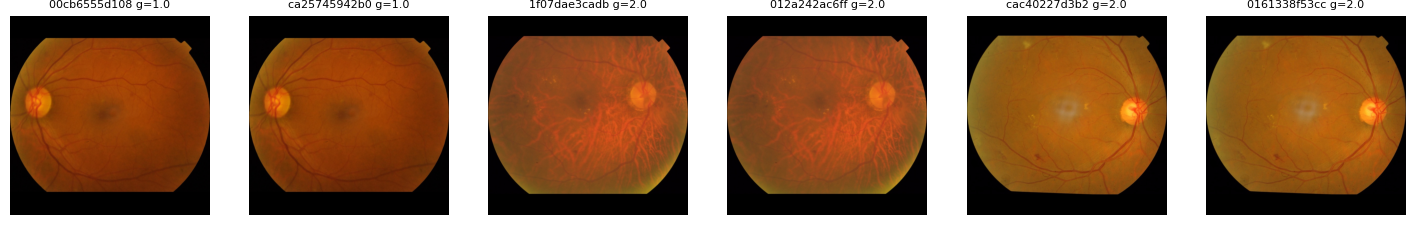
\includegraphics[width=\linewidth]{fig_dups.png}
\caption{APTOS near-duplicate pairs found by perceptual hashing (adjacent images belong to one group). Groups with conflicting grades were removed.}
\label{fig:dups}
\end{figure}

\subsection{Splits}
We hold out 10\% of the labelled training pool as validation. The split is grouped by patient (both eyes of an EyePACS patient, or one APTOS duplicate group, stay together) and stratified by dataset $\times$ grade, using \texttt{StratifiedGroupKFold}.
Validation keeps the natural class mix, which matters because all thresholds are tuned on it. It is used for checkpoint selection, threshold tuning and fusion fitting.
The EyePACS test and Messidor-2 sets are used only for reporting.
Table~\ref{tab:grades} shows the grade distribution.

\begin{table}[t]
\centering\caption{Images per grade after cleaning.}\label{tab:grades}
\footnotesize
\setlength{\tabcolsep}{4pt}
\begin{tabular}{@{}lrrrrrr@{}}
\toprule
Split & 0 & 1 & 2 & 3 & 4 & Total\\
\midrule
Train & 24,864 & 2,509 & 5,590 & 907 & 877 & 34,747\\
Val & 2,739 & 270 & 623 & 134 & 95 & 3,861\\
EyePACS test & 39,529 & 3,762 & 7,860 & 1,214 & 1,206 & 53,571\\
Messidor-2 & 1,017 & 270 & 347 & 75 & 35 & 1,744\\
\midrule
Train share & 71.6\% & 7.2\% & 16.1\% & 2.6\% & 2.5\% & \\
\bottomrule
\end{tabular}
\end{table}

\section{Method}
\subsection{Backbones}
\textbf{ViT-B/16} (\path{vit_base_patch16_384.augreg_in21k_ft_in1k}~\cite{augreg}) is fine-tuned at 512\,px, which gives 1024 tokens. Its learned position embeddings are bicubically resampled from the 24$\times$24 grid to 32$\times$32.
\textbf{ResNet-50} (\path{resnet50.a1_in1k}~\cite{resnet}) is the CNN baseline, the same architecture that Huang \emph{et al.}~\cite{huang} tuned on this task.
Both come from \texttt{timm}~\cite{timm}. Their classifier is replaced by a 4-output linear head.

\subsection{Ordinal formulation and loss}\label{sec:loss}
For grade $y\in\{0,\dots,4\}$ the head outputs logits $z_k$, $k=0..3$, modelling $P(y>k)=\sigma(z_k)$~\cite{frankhall,coral}.
The targets $t_k=\mathbb{1}[y>k]$ are smoothed towards 0.5 to absorb label noise~\cite{smoothing}:
\begin{equation}
\tilde t_k = (1-\epsilon)\,t_k + \epsilon/2,\qquad \epsilon = 0.05,
\end{equation}
and trained with the mean binary cross-entropy over the four outputs.
The continuous score is the expected grade,
\begin{equation}
s = \mathbb{E}[y] = \sum_{k=0}^{3} P(y>k) = \sum_{k=0}^{3}\sigma(z_k)\in[0,4].
\end{equation}
Mistakes between distant grades therefore move $s$ further than mistakes between neighbouring grades, as the quadratic weighting of QWK requires.
Like the regression objectives favoured by~\cite{huang}, $s$ can then be cut at learned thresholds.

\subsection{Class imbalance}
Each training image is sampled with probability proportional to $n_{y}^{-\alpha}$, where $n_y$ is the size of its class, with $\alpha=0.5$ (square-root rebalancing~\cite{kang}).
Here $\alpha=0$ is natural sampling and $\alpha=1$ is fully class-balanced.
This roughly halves grade 0's share and quadruples PDR's, without the extreme repetition of fully balanced sampling, which overfits rare grades~\cite{huang}.
Because the sampled distribution differs from deployment, the decision thresholds are re-fitted on the naturally distributed validation set. We also audit bias with per-grade recall and predicted-vs.-true grade counts.

\subsection{Training}
Both models are trained for 10 epochs with the settings in Table~\ref{tab:hparams}.
\begin{itemize}
\item \textbf{Optimiser:} AdamW~\cite{adamw} (weight decay 0.05) with a one-cycle schedule~\cite{onecycle} (10\% warm-up, cosine decay). The head uses a 10$\times$ learning rate.
\item \textbf{Precision and stability:} fp16 mixed precision~\cite{amp} with gradient clipping at 1.0.
\item \textbf{Augmentation:} random rotation (0--360\textdegree), scale 0.95--1.1, horizontal flip and exposure jitter (contrast 0.8--1.2, brightness $\pm$20), applied before enhancement.
\item \textbf{Checkpoint selection:} after each epoch the model is scored on validation without TTA, and the checkpoint with the best QWK is kept.
\end{itemize}

\begin{table}[t]
\centering\caption{Training configuration (both models).}\label{tab:hparams}
\footnotesize
\begin{tabular}{@{}lll@{}}
\toprule
 & ViT-B/16 & ResNet-50\\
\midrule
Input / preprocessing & \multicolumn{2}{c}{512\,px, Ben Graham, disc mask}\\
Batch / epochs & \multicolumn{2}{c}{16 (8 per GPU) / 10}\\
Backbone LR (head $\times$10) & $5\times10^{-5}$ & $1\times10^{-4}$\\
Sampling $\alpha$ / smoothing $\epsilon$ & \multicolumn{2}{c}{0.5 / 0.05}\\
Pretraining & IN-21k$\rightarrow$IN-1k (AugReg) & IN-1k (A1)\\
Parameters & 86\,M & 24\,M\\
\bottomrule
\end{tabular}
\end{table}

\subsection{Test-time augmentation and uncertainty}
At test time each image is scored in four views: identity, horizontal flip, vertical flip and 180\textdegree\ rotation.
The mean of the four scores is the prediction. Their standard deviation measures how unstable the prediction is.
Images above the 95th percentile of the validation spread are flagged for human review.

\subsection{Operating points}
\textbf{Grading.} The cut-offs $\theta_1<\dots<\theta_4$ on $s$ are fitted on validation by coordinate ascent on QWK: three sweeps of a 39-point grid per threshold, each bounded by its neighbours. This is the ``optimised rounder'' used by APTOS-2019 solutions.
\textbf{Screening.} A referral rule needs high sensitivity rather than maximal kappa, so we fix a separate cut-off $\tau$ on $s$. $\tau$ is the lower 10th percentile of validation scores of truly referable images, so validation rDR sensitivity is at least 90\%.
Per patient, the patient is referred if either eye exceeds $\tau$.

\subsection{Ensemble and paired-eye fusion}
The \emph{ensemble} averages the expected-grade scores of the ViT and the ResNet-50.
\emph{Paired-eye fusion} exploits the strong correlation between a patient's two eyes~\cite{graham,huang}. A linear model is fitted on validation:
\begin{equation}
\hat s_i = w_1 s_i + w_2 s_{\bar i} + b,
\end{equation}
where $\bar i$ is the patient's other eye. For unpaired images (APTOS, Messidor-2) the image's own score is used twice.
The fitted weights are $w=(0.776, 0.307)$ for the ensemble and $(0.709, 0.354)$ for the ViT alone. The other eye thus carries about 30\% of the evidence.
The cut-offs are then re-fitted on validation, and the final variant is chosen by validation QWK.

\subsection{Multi-GPU training on Kaggle}\label{sec:ddp}
Our first runs used \texttt{nn.DataParallel} on the two T4s, and both models came out unexpectedly slow (Table~\ref{tab:compute}).
\begin{itemize}
\item The ViT trained at 24\,img/s, and at 19\,img/s once \texttt{cudnn.benchmark} was enabled.
\item ResNet-50, about 5$\times$ cheaper per image, trained at only 16\,img/s with 0\% data-loader wait.
\item Host RAM grew linearly from 12\% to 88\% over the run, and the kernel was killed during test evaluation. An earlier CNN attempt ran at 2.6\,img/s and died within 30 minutes.
\end{itemize}
The cause is the interaction of two mechanisms. \texttt{DataParallel} launches fresh Python threads on every forward pass, while cuDNN v8 execution plans in PyTorch are cached \emph{per thread}~\cite{prcache}.
Every convolution is therefore re-planned (or re-benchmarked) on every step, and the plans accumulate in host memory. Networks with many convolutions suffer most, while a ViT has only one.
The released code replaces \texttt{DataParallel} with DistributedDataParallel~\cite{ddp}: one forked process per GPU, rank-seeded weighted sampling, rank-0 validation, and TTA inference sharded across GPUs.
It also limits each forked process to one OpenMP thread, which avoids a libgomp deadlock after \texttt{fork}.
This version passes an end-to-end CPU test with two processes. However, the results in this paper come from the \texttt{DataParallel} runs, which are numerically valid but slow, since we did not have the GPU quota to re-train.

\section{Experimental Setup}
\textbf{Metrics.}
\begin{itemize}
\item QWK~\cite{cohen}: $\kappa = 1-\frac{\sum_{ij} w_{ij} O_{ij}}{\sum_{ij} w_{ij} E_{ij}}$ with $w_{ij}=(i-j)^2/16$, where $O$ is the observed and $E$ the chance-expected confusion matrix.
\item Accuracy and macro-averaged per-grade recall.
\item rDR and VTDR AUC from the continuous score.
\item rDR sensitivity and specificity at the QWK cut-offs and at the screening cut-off $\tau$.
\end{itemize}
95\% confidence intervals come from a non-parametric bootstrap~\cite{bootstrap}: 500 resamples for single models and 300 for the fusion variants.
\textbf{Protocol.} Everything that is fitted (checkpoint, cut-offs, $\tau$, uncertainty cut-off, fusion weights, final-variant choice) is fitted on validation. EyePACS test and Messidor-2 are scored once.
Literature comparisons use the Kaggle Private split, which has 42,670 images; ours has 4 fewer because those images had no detectable fundus.

\section{Results}
\subsection{Training dynamics and compute}
Fig.~\ref{fig:curves} shows validation QWK and training loss.
The ViT fits the training data faster (final loss 0.21 vs.\ 0.29), and its validation QWK peaks at 0.827 in epoch~8.
The ResNet-50 peaks at 0.811 in epoch~7. Both plateau after about 7 epochs with the one-cycle schedule.
Table~\ref{tab:compute} lists wall-clock costs: 5.5--6.3\,h of training per model, so about 12 GPU-hours for the final two-model system plus evaluation.

\begin{figure*}[t]
\centering
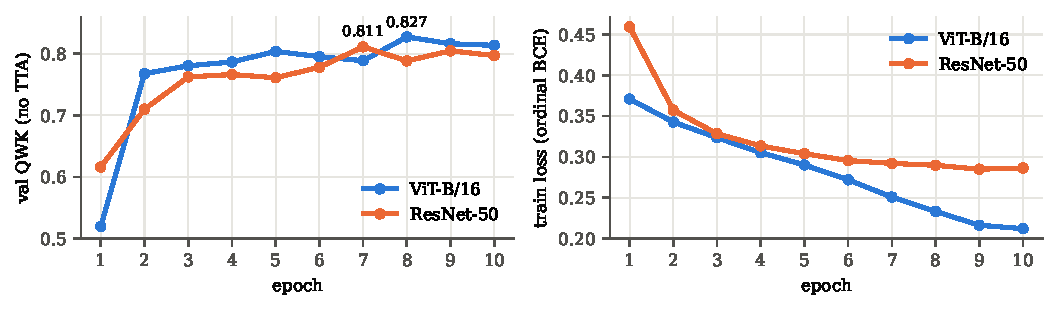
\includegraphics[width=0.92\linewidth]{fig_curves.pdf}
\caption{Validation QWK (single view, default cut-offs) and training loss per epoch. Labels mark the selected checkpoints.}
\label{fig:curves}
\end{figure*}

\begin{table}[t]
\centering\caption{Compute on Kaggle 2$\times$T4 (\texttt{DataParallel} runs).}\label{tab:compute}
\footnotesize
\setlength{\tabcolsep}{3pt}
\begin{tabular}{@{}lrrr@{}}
\toprule
Run & img/s & train time & host RAM\\
\midrule
Preprocessing (CPU only) & -- & $\sim$1--2\,h & --\\
ViT-B/16, run 1 & 24 & 4.4\,h & n/a\\
ViT-B/16, run 2 (cuDNN benchmark) & 19 & 5.5\,h & 12$\rightarrow$16\%\\
ResNet-50 & 16 & 6.3\,h & 12$\rightarrow$88\%$^\dagger$\\
Fusion + ensemble (CPU only) & -- & minutes & --\\
\bottomrule
\multicolumn{4}{@{}l@{}}{\scriptsize $^\dagger$kernel killed during test evaluation; evaluation re-run from the checkpoint.}
\end{tabular}
\end{table}

\subsection{Main results}
Table~\ref{tab:main} and Fig.~\ref{fig:variants} compare all variants.
\begin{itemize}
\item \textbf{Single models} are close on EyePACS: ViT 0.808 vs.\ ResNet-50 0.803 on the Private split (CIs overlap, $\pm$0.005).
\item \textbf{Paired-eye fusion} is the largest single improvement: +0.022 QWK for the ViT and +0.016 for the ResNet-50 on Private. It also raises rDR AUC (ViT 0.937$\rightarrow$0.950).
\item \textbf{The ensemble} of the two backbones adds +0.010 over the ViT.
\item \textbf{Combined}, ensemble + pair reaches 0.838 Private QWK and rDR AUC 0.955. It is the variant with the best validation QWK (0.864), so we select it as the final model.
\end{itemize}

\begin{table*}[t]
\centering
\caption{Results of all variants. QWK and rDR metrics on validation, the EyePACS Private test (n=42,666) and the external Messidor-2 set (n=1,744). ``screen'' = screening cut-off $\tau$ fixed at 90\% val rDR sensitivity. Bold: best per column (excluding val).}
\label{tab:main}
\footnotesize
\setlength{\tabcolsep}{4.2pt}
\begin{tabular}{@{}l c ccccc ccccc@{}}
\toprule
& Val & \multicolumn{5}{c}{EyePACS Private test} & \multicolumn{5}{c}{Messidor-2 (external)}\\
\cmidrule(lr){3-7}\cmidrule(lr){8-12}
Variant & QWK & QWK & rDR AUC & sens$_{\text{screen}}$ & spec$_{\text{screen}}$ & VTDR AUC & QWK & rDR AUC & sens$_{\text{screen}}$ & spec$_{\text{screen}}$ & VTDR AUC\\
\midrule
ViT-B/16 & 0.843 & 0.808 & 0.937 & \textbf{0.873} & 0.876 & 0.966 & 0.840 & 0.964 & 0.956 & 0.781 & 0.988\\
ResNet-50 & 0.834 & 0.803 & 0.937 & \textbf{0.878} & 0.861 & 0.970 & 0.819 & 0.958 & \textbf{0.980} & 0.608 & 0.989\\
Ensemble & 0.852 & 0.818 & 0.947 & 0.872 & 0.904 & 0.973 & \textbf{0.853} & \textbf{0.969} & 0.974 & 0.743 & \textbf{0.992}\\
ViT + pair & 0.860 & 0.830 & 0.950 & 0.858 & \textbf{0.934} & 0.974 & 0.831 & 0.964 & 0.943 & \textbf{0.848} & 0.988\\
ResNet-50 + pair & 0.848 & 0.819 & 0.947 & 0.861 & 0.911 & 0.974 & 0.800 & 0.958 & 0.972 & 0.702 & 0.989\\
\textbf{Ensemble + pair} & \textbf{0.864} & \textbf{0.838} & \textbf{0.955} & 0.865 & 0.932 & \textbf{0.977} & 0.843 & \textbf{0.969} & 0.956 & 0.791 & \textbf{0.992}\\
\bottomrule
\end{tabular}
\end{table*}

\begin{figure*}[t]
\centering
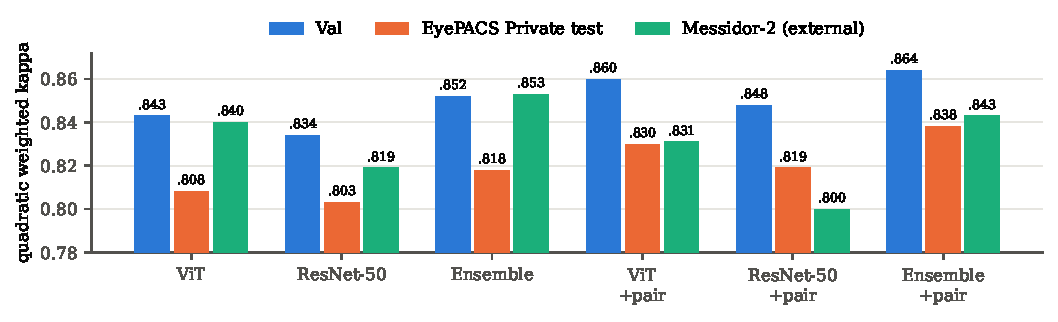
\includegraphics[width=0.92\linewidth]{fig_variants.pdf}
\caption{QWK of every variant on validation, the EyePACS Private test and the external Messidor-2 set. Paired-eye fusion helps on EyePACS (where both eyes are available) but not on Messidor-2, where unpaired images receive their own score twice.}
\label{fig:variants}
\end{figure*}

Table~\ref{tab:final} gives the final model with confidence intervals.
At the QWK cut-offs the model is conservative: rDR sensitivity is 0.725 and specificity 0.983.
The screening cut-off moves it to 86.5\% sensitivity and 93.2\% specificity on the Private test, and 95.6\% / 79.1\% on Messidor-2.
On the EyePACS test set, patient-level referral (the worse eye decides) raises sensitivity by about 3 points for single models, e.g.\ ViT test 0.874$\rightarrow$0.901, at a cost of about 6 points of specificity.

\begin{table}[t]
\centering\caption{Final model (ensemble + paired-eye fusion) with 95\% bootstrap CIs.}\label{tab:final}
\footnotesize
\setlength{\tabcolsep}{3pt}
\begin{tabular}{@{}lll@{}}
\toprule
Metric & EyePACS Private & Messidor-2 (external)\\
\midrule
QWK & 0.838 \pmci{0.834}{0.843} & 0.843 \pmci{0.825}{0.861}\\
Accuracy & 0.804 \pmci{0.800}{0.807} & 0.727 \pmci{0.705}{0.746}\\
Macro recall & 0.591 \pmci{0.581}{0.600} & 0.663 \pmci{0.622}{0.700}\\
rDR AUC & 0.955 \pmci{0.952}{0.957} & 0.969 \pmci{0.960}{0.978}\\
rDR sens / spec @QWK & 0.725 / 0.983 & 0.895 / 0.934\\
rDR sens @screen & 0.865 \pmci{0.857}{0.873} & 0.956 \pmci{0.935}{0.974}\\
rDR spec @screen & 0.932 \pmci{0.929}{0.934} & 0.791 \pmci{0.772}{0.814}\\
VTDR AUC & 0.977 \pmci{0.973}{0.979} & 0.992 \pmci{0.987}{0.995}\\
\bottomrule
\end{tabular}
\end{table}

\subsection{Per-grade behaviour and bias}
Fig.~\ref{fig:cm} shows the confusion matrices of the final model and Fig.~\ref{fig:recall} the recall per grade.
\begin{itemize}
\item \textbf{Errors are almost all between adjacent grades.} On the Private test only 3 of 31,400 grade-0 images (0.01\%) are called PDR, and 0.9\% of PDR images are called grade 0.
\item \textbf{Grade 0} is recognised well (recall 0.93).
\item \textbf{Mild DR} is the weakest class (0.37). It is also where human graders disagree most~\cite{krause}: an isolated microaneurysm at 512\,px is close to the noise floor.
\item \textbf{Moderate DR} has the largest absolute error mass. Of 6,281 Private images, 22\% are called mild and 19\% severe.
\item \textbf{Severe NPDR is over-predicted} (2,248 predicted vs.\ 977 true on Private). This is a direct consequence of $\alpha=0.5$ oversampling combined with QWK-optimal cut-offs: QWK penalises an under-call of a PDR image more than an over-call of a moderate one.
\item \textbf{Bias across grades is limited.} Predicted grade frequencies stay within a factor of 2.3 of the true ones for every grade, and the macro recall of 0.59 is far above the 0.20 of a majority-class predictor.
\item \textbf{Across sources}, validation QWK is 0.918 (ViT) / 0.893 (CNN) on APTOS vs.\ 0.828 / 0.819 on EyePACS. APTOS images are more homogeneous, so the pooled validation score overstates EyePACS performance, and we report the sources separately.
\end{itemize}

\begin{figure*}[t]
\centering
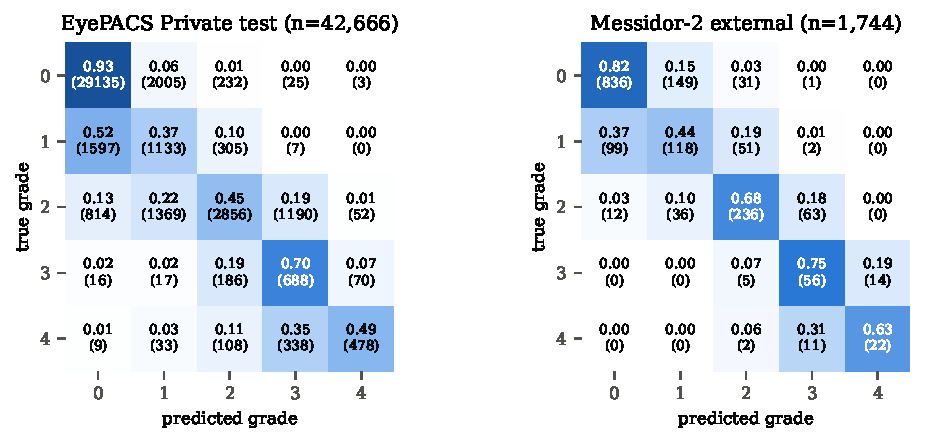
\includegraphics[width=0.8\linewidth]{fig_cm.pdf}
\caption{Confusion matrices of the final model, row-normalised (counts in parentheses). Errors concentrate next to the diagonal; mild DR and the moderate/severe boundary are the main confusions.}
\label{fig:cm}
\end{figure*}

\begin{figure*}[t]
\centering
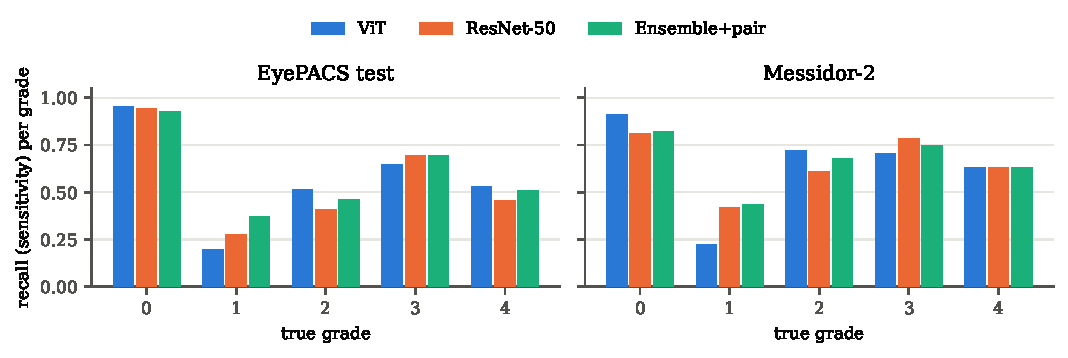
\includegraphics[width=0.92\linewidth]{fig_recall.pdf}
\caption{Recall per grade for the single models and the final model (EyePACS: full 53,571-image test set). The ensemble mostly improves mild DR; the ViT is the stronger single model on Messidor-2 for grades 0 and 2.}
\label{fig:recall}
\end{figure*}

\subsection{External validation and domain shift}
On Messidor-2, a different country, camera and grading protocol, QWK is \emph{not} lower than on EyePACS (0.843 vs.\ 0.838).
This is plausible for two reasons. Messidor-2 images are of uniformly good quality, and its reference grades are adjudicated by three retina specialists rather than given by one grader, so less of the measured error comes from label noise.
The architectures differ clearly here, however.
\begin{itemize}
\item The \textbf{ViT transfers better} than the ResNet-50: QWK 0.840 \pmci{0.819}{0.858} vs.\ 0.819 \pmci{0.796}{0.839}, and rDR AUC 0.964 vs.\ 0.958.
\item The \textbf{CNN's scores shift upward} on the new camera. Its screening cut-off, calibrated on EyePACS/APTOS validation, keeps 98\% sensitivity but drops to \textbf{0.608 specificity}, against 0.781 for the ViT. Grade 0 recall falls to 0.81, against 0.91 for the ViT (Fig.~\ref{fig:recall}).
\item \textbf{Paired-eye fusion does not help on Messidor-2} (ViT 0.840$\rightarrow$0.831), because its images are unpaired in our data. Using the own score twice just rescales it by $w_1+w_2\approx1.07$, which shifts it against cut-offs fitted on paired EyePACS images.
\end{itemize}
A model that ranks well (high AUC) can still mis-place its operating point on a new site. The cut-off of a screening deployment must therefore be re-calibrated on local images (Sec.~\ref{sec:limits}).

\subsection{TTA-based uncertainty}
Flagging the 5\% of images with the largest TTA spread for human review works as intended. On the remaining images, QWK rises:
\begin{itemize}
\item EyePACS test: ViT 0.808$\rightarrow$0.824 (4.9\% flagged), ResNet-50 0.804$\rightarrow$0.819 (5.1\% flagged).
\item Messidor-2: ViT 0.840$\rightarrow$0.856 (7.0\% flagged), ResNet-50 0.819$\rightarrow$0.854 (9.9\% flagged).
\end{itemize}
More images are flagged on the external set, consistent with domain shift, so the flag is a useful though uncalibrated safety valve.

\subsection{Reproducibility}
Two ViT runs with identical hyper-parameters gave nearly the same result on EyePACS.
The second run differed only in \texttt{cudnn.benchmark} and in non-deterministic kernels.
\begin{itemize}
\item EyePACS test: QWK 0.809 and 0.808; rDR AUC 0.936 and 0.937.
\item Messidor-2: QWK 0.811 and 0.840.
\end{itemize}
The external spread (0.03) is larger than the bootstrap CI, so single-run external comparisons between architectures should be read with that seed variance in mind.

\subsection{Comparison with the literature}
Table~\ref{tab:sota} places our results among published ones.
On the EyePACS Private test our single 512\,px models (0.803--0.808) are about 0.02--0.03 below the carefully tuned ResNet-50 of Huang \emph{et al.} (0.831). That model trained for 25 epochs, without Ben enhancement and with instance-balanced sampling; each of those differences favoured it in their ablation.
Our final system (0.838) is 0.011--0.025 below the published state of the art (0.849--0.863).
On Messidor-2 our rDR AUC of 0.969 clearly exceeds the public-data reproduction of Voets \emph{et al.} (0.853) and approaches Gulshan \emph{et al.} (0.990), who trained on 128k multiply-graded private images.
These AUCs are not strictly comparable because the reference grades differ: ours are the adjudicated grades of~\cite{krause}.

\begin{table}[t]
\centering\caption{Comparison with published results. Top: QWK on the Kaggle EyePACS Private test (values from~\cite{huang}). Bottom: rDR AUC on Messidor-2 for models not trained on Messidor.}\label{tab:sota}
\footnotesize
\begin{tabular}{@{}llr@{}}
\toprule
Method & Notes & QWK\\
\midrule
Min-Pooling (Graham)~\cite{graham} & Kaggle winner, both eyes & 0.849\\
o\_O (Kaggle 2nd) & both eyes & 0.845\\
Zoom-in-Net~\cite{zoomin} & lesion attention & 0.854\\
AFN~\cite{afn} & lesion detector & 0.859\\
CABNet~\cite{cabnet} & ResNet-50 & 0.846\\
Huang \emph{et al.}~\cite{huang} & ResNet-50, single eye & 0.831\\
Huang \emph{et al.}~\cite{huang} & + paired fusion / ensemble & 0.858 / 0.863\\
\midrule
Ours, ViT-B/16 & single eye, 10 epochs & 0.808\\
Ours, ResNet-50 & single eye, 10 epochs & 0.803\\
Ours, ensemble + pair & final & 0.838\\
\midrule
 & & rDR AUC\\
\midrule
Gulshan \emph{et al.}~\cite{gulshan} & 128k private images & 0.990\\
Voets \emph{et al.}~\cite{voets} & public EyePACS only & 0.853\\
Ours, final & EyePACS + APTOS & 0.969\\
\bottomrule
\end{tabular}
\end{table}

\section{Discussion}
\textbf{CNN vs.\ ViT.} With identical training, a ViT-B/16 at 512\,px matches a ResNet-50 at 512\,px on in-distribution data. It needs about 3.6$\times$ the parameters and many more FLOPs per image, but it generalises better to an unseen camera.
The two make different errors: the ensemble improves on both, and helps mild-DR recall most.
Under a fixed GPU budget the CNN's cheaper per-image cost could be spent on 768\,px inputs (+0.01 QWK in~\cite{huang}). A ViT at 768\,px (2,304 tokens) does not fit a T4 budget.

\textbf{What we would change.}
The literature~\cite{huang} and our confusion matrices point to four inexpensive ablations that we could not run within the remaining quota:
\begin{enumerate}
\item no Ben enhancement for pretrained backbones;
\item natural sampling ($\alpha=0$), which should reduce the severe-grade over-prediction;
\item a 768\,px CNN;
\item feature-level, rather than score-level, paired-eye fusion.
\end{enumerate}
The DDP fix (Sec.~\ref{sec:ddp}) makes all of these several times cheaper for CNNs.

\section{Clinical Limitations}\label{sec:limits}
\begin{enumerate}
\item \textbf{Not a medical device.} This is a retrospective research prototype without prospective validation or regulatory clearance. It should be used as a triage aid that prioritises human grading.
\item \textbf{Label quality.} EyePACS labels come from single graders, and mild DR is unreliable for humans and model alike (recall 0.37--0.44).
\item \textbf{Domain shift.} The training images come from the USA and India, and the external evaluation from France. The CNN example shows that a cut-off can lose 25 points of specificity on a new camera even when AUC stays high. Before deployment, the referral cut-off must be validated and re-calibrated on local images from the camps' own (often hand-held, non-mydriatic) cameras.
\item \textbf{No image-quality model.} The tool rejects only images without a detectable fundus disc. Blurred, dark or off-centre images still receive a grade. Deployments reject a substantial share of field images as ungradable~\cite{beede}, so a gradeability check and a human fallback are required.
\item \textbf{Scope.} The tool grades DR only. It does not detect diabetic macular oedema, which can threaten vision at any DR grade, nor glaucoma, AMD or vein occlusions. ``No DR'' therefore does not mean a normal eye.
\item \textbf{Single 45\textdegree\ field.} Peripheral lesions outside the photographed field are invisible, unlike in the ETDRS 7-field reference standard.
\item \textbf{Operating point.} The QWK-optimal cut-offs give only 73\% rDR sensitivity on EyePACS. Referral must use the screening cut-off: 86.5\% sensitivity at 93.2\% specificity on the Private test, which is comparable in magnitude to IDx-DR's prospective 87.2\% / 90.7\%~\cite{abramoff}. The protocols differ, so this is not a head-to-head comparison.
\item \textbf{Uncertainty.} The TTA flag is not calibrated; confidently wrong predictions remain possible.
\item \textbf{Fairness.} None of the datasets provide age, sex or ethnicity, so subgroup performance cannot be audited. Our bias checks are limited to per-grade recall and per-source performance.
\end{enumerate}

\section{Conclusion}
We presented a free-tier, end-to-end DR grading pipeline. It runs on the original 82\,GB EyePACS archive, cleans noisy labels, and trains ordinal ViT and CNN graders at 512\,px.
It reports internal and external results with per-grade confusion matrices and two operating points.
A two-model ensemble with paired-eye fusion reaches QWK 0.838 on the EyePACS Private test and 0.843 on the external Messidor-2 set, with referable-DR AUC 0.955 and 0.969.
The ViT is not more accurate than the CNN in-distribution, but it transfers better to a new site.
For screening, the main lesson is that calibrating the operating point on local data matters as much as the choice of architecture.

\section*{Team Contributions}
\begin{itemize}
\item S.~Shakya: coordination, pipeline integration, multi-GPU engineering.
\item A.~Shukla: data access and verification.
\item A.~Kumar: streaming preprocessing.
\item N.~Gupta: EDA, deduplication, splits.
\item U.~Kumar: ViT and ordinal head.
\item A.~Usara: ResNet-50 and imbalance sampling.
\item S.~Gupta: metrics, thresholds, CIs.
\item K.~K.~Gupta: external validation, TTA and uncertainty.
\item S.~Mishra: ensemble, paired-eye fusion, screening tool.
\item S.~Anand: literature, clinical limitations, report.
\end{itemize}

\begin{thebibliography}{99}
\footnotesize
\bibitem{teo} Z.~L. Teo \emph{et al.}, ``Global prevalence of diabetic retinopathy and projection of burden through 2045: Systematic review and meta-analysis,'' \emph{Ophthalmology}, vol.~128, no.~11, pp.~1580--1591, 2021.
\bibitem{gulshan} V.~Gulshan \emph{et al.}, ``Development and validation of a deep learning algorithm for detection of diabetic retinopathy in retinal fundus photographs,'' \emph{JAMA}, vol.~316, no.~22, pp.~2402--2410, 2016.
\bibitem{krause} J.~Krause \emph{et al.}, ``Grader variability and the importance of reference standards for evaluating machine learning models for diabetic retinopathy,'' \emph{Ophthalmology}, vol.~125, no.~8, pp.~1264--1272, 2018.
\bibitem{abramoff} M.~D. Abr\`amoff, P.~T. Lavin, M.~Birch, N.~Shah, and J.~C. Folk, ``Pivotal trial of an autonomous AI-based diagnostic system for detection of diabetic retinopathy in primary care offices,'' \emph{npj Digit. Med.}, vol.~1, art.~39, 2018.
\bibitem{beede} E.~Beede \emph{et al.}, ``A human-centered evaluation of a deep learning system deployed in clinics for the detection of diabetic retinopathy,'' in \emph{Proc. CHI}, 2020.
\bibitem{icdr} C.~P. Wilkinson \emph{et al.}, ``Proposed international clinical diabetic retinopathy and diabetic macular edema disease severity scales,'' \emph{Ophthalmology}, vol.~110, no.~9, pp.~1677--1682, 2003.
\bibitem{cohen} J.~Cohen, ``Weighted kappa: Nominal scale agreement with provision for scaled disagreement or partial credit,'' \emph{Psychol. Bull.}, vol.~70, no.~4, pp.~213--220, 1968.
\bibitem{voets} M.~Voets, K.~M{\o}llersen, and L.~A. Bongo, ``Reproduction study using public data of: Development and validation of a deep learning algorithm for detection of diabetic retinopathy in retinal fundus photographs,'' \emph{PLoS ONE}, vol.~14, no.~6, e0217541, 2019.
\bibitem{graham} B.~Graham, ``Kaggle diabetic retinopathy detection competition report,'' University of Warwick, Tech. Rep., 2015.
\bibitem{zoomin} Z.~Wang, Y.~Yin, J.~Shi, W.~Fang, H.~Li, and X.~Wang, ``Zoom-in-Net: Deep mining lesions for diabetic retinopathy detection,'' in \emph{Proc. MICCAI}, 2017.
\bibitem{afn} Z.~Lin \emph{et al.}, ``A framework for identifying diabetic retinopathy based on anti-noise detection and attention-based fusion,'' in \emph{Proc. MICCAI}, 2018.
\bibitem{cabnet} A.~He, T.~Li, N.~Li, K.~Wang, and H.~Fu, ``CABNet: Category attention block for imbalanced diabetic retinopathy grading,'' \emph{IEEE Trans. Med. Imaging}, vol.~40, no.~1, pp.~143--153, 2021.
\bibitem{huang} Y.~Huang, L.~Lin, P.~Cheng, J.~Lyu, R.~Tam, and X.~Tang, ``Identifying the key components in ResNet-50 for diabetic retinopathy grading from fundus images: A systematic investigation,'' arXiv:2110.14160, 2021.
\bibitem{frankhall} E.~Frank and M.~Hall, ``A simple approach to ordinal classification,'' in \emph{Proc. ECML}, 2001, pp.~145--156.
\bibitem{coral} W.~Cao, V.~Mirjalili, and S.~Raschka, ``Rank consistent ordinal regression for neural networks with application to age estimation,'' \emph{Pattern Recognit. Lett.}, vol.~140, pp.~325--331, 2020.
\bibitem{kang} B.~Kang \emph{et al.}, ``Decoupling representation and classifier for long-tailed recognition,'' in \emph{Proc. ICLR}, 2020.
\bibitem{smoothing} R.~M{\"u}ller, S.~Kornblith, and G.~Hinton, ``When does label smoothing help?'' in \emph{Proc. NeurIPS}, 2019.
\bibitem{vit} A.~Dosovitskiy \emph{et al.}, ``An image is worth 16x16 words: Transformers for image recognition at scale,'' in \emph{Proc. ICLR}, 2021.
\bibitem{augreg} A.~Steiner \emph{et al.}, ``How to train your ViT? Data, augmentation, and regularization in vision transformers,'' \emph{Trans. Mach. Learn. Res.}, 2022.
\bibitem{lat} R.~Sun, Y.~Li, T.~Zhang, Z.~Mao, F.~Wu, and Y.~Zhang, ``Lesion-aware transformers for diabetic retinopathy grading,'' in \emph{Proc. CVPR}, 2021.
\bibitem{retfound} Y.~Zhou \emph{et al.}, ``A foundation model for generalizable disease detection from retinal images,'' \emph{Nature}, vol.~622, pp.~156--163, 2023.
\bibitem{eyepacs} J.~Cuadros and G.~Bresnick, ``EyePACS: An adaptable telemedicine system for diabetic retinopathy screening,'' \emph{J. Diabetes Sci. Technol.}, vol.~3, no.~3, pp.~509--516, 2009.
\bibitem{messidor} E.~Decenci\`ere \emph{et al.}, ``Feedback on a publicly distributed image database: The Messidor database,'' \emph{Image Anal. Stereol.}, vol.~33, no.~3, pp.~231--234, 2014.
\bibitem{zauner} C.~Zauner, ``Implementation and benchmarking of perceptual image hash functions,'' M.S. thesis, Upper Austria Univ. Appl. Sci., 2010.
\bibitem{resnet} K.~He, X.~Zhang, S.~Ren, and J.~Sun, ``Deep residual learning for image recognition,'' in \emph{Proc. CVPR}, 2016.
\bibitem{timm} R.~Wightman, ``PyTorch image models,'' GitHub repository, \url{https://github.com/huggingface/pytorch-image-models}, 2019.
\bibitem{adamw} I.~Loshchilov and F.~Hutter, ``Decoupled weight decay regularization,'' in \emph{Proc. ICLR}, 2019.
\bibitem{onecycle} L.~N. Smith and N.~Topin, ``Super-convergence: Very fast training of neural networks using large learning rates,'' in \emph{Proc. SPIE}, vol.~11006, 2019.
\bibitem{amp} P.~Micikevicius \emph{et al.}, ``Mixed precision training,'' in \emph{Proc. ICLR}, 2018.
\bibitem{bootstrap} B.~Efron and R.~J. Tibshirani, \emph{An Introduction to the Bootstrap}. Chapman \& Hall, 1993.
\bibitem{ddp} S.~Li \emph{et al.}, ``PyTorch distributed: Experiences on accelerating data parallel training,'' \emph{Proc. VLDB Endow.}, vol.~13, no.~12, 2020.
\bibitem{prcache} PyTorch contributors, ``[cuDNN][cuDNN V8 API] Share benchmarked conv plans across threads,'' pull request \#191744, \url{https://github.com/pytorch/pytorch/pull/191744}.
\end{thebibliography}
\end{document}
